% Options for packages loaded elsewhere
\PassOptionsToPackage{unicode}{hyperref}
\PassOptionsToPackage{hyphens}{url}
%
\documentclass[
]{book}
\usepackage{amsmath,amssymb}
\usepackage{lmodern}
\usepackage{ifxetex,ifluatex}
\ifnum 0\ifxetex 1\fi\ifluatex 1\fi=0 % if pdftex
  \usepackage[T1]{fontenc}
  \usepackage[utf8]{inputenc}
  \usepackage{textcomp} % provide euro and other symbols
\else % if luatex or xetex
  \usepackage{unicode-math}
  \defaultfontfeatures{Scale=MatchLowercase}
  \defaultfontfeatures[\rmfamily]{Ligatures=TeX,Scale=1}
\fi
% Use upquote if available, for straight quotes in verbatim environments
\IfFileExists{upquote.sty}{\usepackage{upquote}}{}
\IfFileExists{microtype.sty}{% use microtype if available
  \usepackage[]{microtype}
  \UseMicrotypeSet[protrusion]{basicmath} % disable protrusion for tt fonts
}{}
\makeatletter
\@ifundefined{KOMAClassName}{% if non-KOMA class
  \IfFileExists{parskip.sty}{%
    \usepackage{parskip}
  }{% else
    \setlength{\parindent}{0pt}
    \setlength{\parskip}{6pt plus 2pt minus 1pt}}
}{% if KOMA class
  \KOMAoptions{parskip=half}}
\makeatother
\usepackage{xcolor}
\IfFileExists{xurl.sty}{\usepackage{xurl}}{} % add URL line breaks if available
\IfFileExists{bookmark.sty}{\usepackage{bookmark}}{\usepackage{hyperref}}
\hypersetup{
  pdftitle={EPI 563: Spatial Epidemiology, Fall 2021},
  pdfauthor={Michael Kramer},
  hidelinks,
  pdfcreator={LaTeX via pandoc}}
\urlstyle{same} % disable monospaced font for URLs
\usepackage{longtable,booktabs,array}
\usepackage{calc} % for calculating minipage widths
% Correct order of tables after \paragraph or \subparagraph
\usepackage{etoolbox}
\makeatletter
\patchcmd\longtable{\par}{\if@noskipsec\mbox{}\fi\par}{}{}
\makeatother
% Allow footnotes in longtable head/foot
\IfFileExists{footnotehyper.sty}{\usepackage{footnotehyper}}{\usepackage{footnote}}
\makesavenoteenv{longtable}
\usepackage{graphicx}
\makeatletter
\def\maxwidth{\ifdim\Gin@nat@width>\linewidth\linewidth\else\Gin@nat@width\fi}
\def\maxheight{\ifdim\Gin@nat@height>\textheight\textheight\else\Gin@nat@height\fi}
\makeatother
% Scale images if necessary, so that they will not overflow the page
% margins by default, and it is still possible to overwrite the defaults
% using explicit options in \includegraphics[width, height, ...]{}
\setkeys{Gin}{width=\maxwidth,height=\maxheight,keepaspectratio}
% Set default figure placement to htbp
\makeatletter
\def\fps@figure{htbp}
\makeatother
\setlength{\emergencystretch}{3em} % prevent overfull lines
\providecommand{\tightlist}{%
  \setlength{\itemsep}{0pt}\setlength{\parskip}{0pt}}
\setcounter{secnumdepth}{5}
\usepackage{color}
\usepackage{framed}
\usepackage{booktabs}
\usepackage{amsmath}
\usepackage{xcolor}
\usepackage{float}

\setlength{\fboxsep}{.8em}

\makeatletter
\def\thm@space@setup{%
  \thm@preskip=8pt plus 2pt minus 4pt
  \thm@postskip=\thm@preskip
}
\makeatother


% Create blackbox 
% \newenvironment{blackbox}{
%   \definecolor{shadecolor}{rgb}{255, 228, 228}  % 255	228	228
%   \color{white}
%   \begin{shaded}}
%  {\end{shaded}}

\usepackage{tcolorbox}
% create rmdcaution based on blackbox
\newtcolorbox{caution}{
  colback=red!50!white,
  colframe=black,
  coltext=black,
  boxsep=5pt,
  arc=4pt}

\newenvironment{rmdcaution}[1]
  {
  \begin{itemize}
  \renewcommand{\labelitemi}{
    \raisebox{-.7\height}[0pt][0pt]{
      {\setkeys{Gin}{width=3em,keepaspectratio}\includegraphics{images/#1}}
    }
  }
  \setlength{\fboxsep}{1em}
  \begin{caution}
  \item
  }
  {
  \end{caution}
  \end{itemize}
  }
  
  
  % create rmdnote based on blackbox
\newtcolorbox{note}{
  colback=black!5!white,
  colframe=black,
  coltext=black,
  boxsep=5pt,
  arc=4pt}

\newenvironment{rmdnote}[1]
  {
  \begin{itemize}
  \renewcommand{\labelitemi}{
    \raisebox{-.7\height}[0pt][0pt]{
      {\setkeys{Gin}{width=3em,keepaspectratio}\includegraphics{images/#1}}
    }
  }
  \setlength{\fboxsep}{1em}
  \begin{note}
  \item
  }
  {
  \end{note}
  \end{itemize}
  }
  
  
  
    % create rmdtip based on blackbox
\newtcolorbox{tip}{
  colback=green!15!white,
  colframe=black,
  coltext=black,
  boxsep=5pt,
  arc=4pt}

\newenvironment{rmdtip}[1]
  {
  \begin{itemize}
  \renewcommand{\labelitemi}{
    \raisebox{-.7\height}[0pt][0pt]{
      {\setkeys{Gin}{width=3em,keepaspectratio}\includegraphics{images/#1}}
    }
  }
  \setlength{\fboxsep}{1em}
  \begin{tip}
  \item
  }
  {
  \end{tip}
  \end{itemize}
  }





\ifluatex
  \usepackage{selnolig}  % disable illegal ligatures
\fi
\usepackage[]{natbib}
\bibliographystyle{apalike}

\title{EPI 563: Spatial Epidemiology, Fall 2021}
\author{Michael Kramer}
\date{Last updated: 2021-08-19}

\begin{document}
\maketitle

{
\setcounter{tocdepth}{1}
\tableofcontents
}
\hypertarget{how-to-use-this-ebook}{%
\chapter*{How to use this eBook}\label{how-to-use-this-ebook}}
\addcontentsline{toc}{chapter}{How to use this eBook}

\begin{center}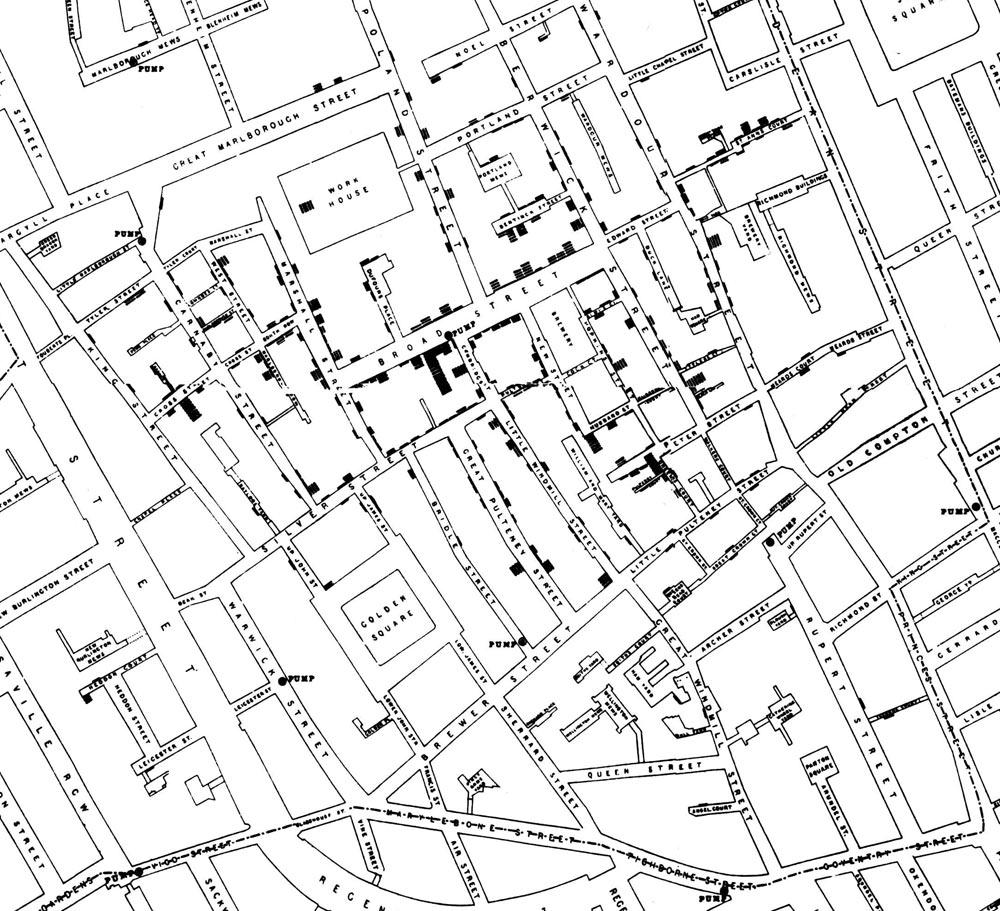
\includegraphics[width=0.5\linewidth]{images/John-Snows-cholera-map-of-009} \end{center}

Welcome to \emph{Concepts \& Applications in Spatial Epidemiology (EPI 563)}! This eBook is one of several sources of information and support for your progress through the semester. For an overview of the course, expectations, learning objectives, assignments, and grading, please review the full course syllabus on Canvas. This eBook serves to provide a \emph{`jumping off point'} for the content to be covered each week. Specifically, the content herein will introduce key themes, new vocabulary, and provide some additional detail that is complementary to the \emph{asynchronous} (pre-recorded) video lectures, and foundational to the \emph{synchronous} (in class) work.

\hypertarget{strategy-for-using-this-ebook}{%
\section*{Strategy for using this eBook}\label{strategy-for-using-this-ebook}}
\addcontentsline{toc}{section}{Strategy for using this eBook}

There is a separate \emph{module} or \emph{chapter} for each week's content. In general, the content within each week's section is divided into two sections focusing on \textbf{spatial thinking} and \textbf{spatial analysis}. This dichotomy does not always hold, but in broad terms you can expect these sections to be more specific to content in class on \emph{Tuesday} versus \emph{Thursday} respectively.

\begin{itemize}
\tightlist
\item
  \emph{Spatial thinking for epidemiology}: This section introduces vocabulary, concepts, and themes that are important to the incorporation of spatialized or geo-referenced data into epidemiologic work. At a minimum, plan to read this content \emph{prior to class Tuesday}, although you will likely benefit from reading both sections before Tuesday.
\item
  \emph{Spatial analysis for epidemiology}: This section is more focused on data management, visualization, spatial statistics, and interpretation. This content is relevant for our work together on Tuesday's, but is essential for successful work in the Thursday lab activities.
\end{itemize}

Throughout the book some concepts or ideas may be highlighted with \emph{call-out blocks}.

\begin{rmdcaution}{caution}
This block denotes a potential pitfall or area of caution.

\end{rmdcaution}

\begin{rmdnote}{note}
This block denotes an additional bit of information or additional idea to \emph{note} about the topic at hand.

\end{rmdnote}

\begin{rmdtip}{tip}
This block denotes a \emph{tip} or advice for best practices or efficiency.

\end{rmdtip}

Please note that I will be continually updating the eBook throughout the semester, so if you choose to download, please double-check the \textbf{Last updated} date to be sure you have the most recent version.


\includegraphics{images/by-nc-sa.png}\\
This eBook is licensed under the \href{http://creativecommons.org/licenses/by-nc-sa/4.0/}{Creative Commons Attribution-NonCommercial-ShareAlike 4.0 International License}.

  \bibliography{book.bib}

\end{document}
